\chapter{Analyse}
\label{chap:anal}
Notre implémentation comprend notamment une représentation binaire, aussi appelé Bitboard, les algorithmes de recherches Minimax et Alpha-Beta, et un classifieur pour prédire le résultat d'une partie en cours. Nous détaillons également les structures de données utilisées, et les algorithmes de décalage pour les coups valides. Nous avons réalisé ce projet en Python, pour des raisons de simplicité et de rapidité de développement, notamment à propos de la visualisation, et du développement du modèle de deep learning via PyTorch\footnote{PyTorch est une bibliothèque de tenseurs optimisée pour l'apprentissage profond. Voir \href{https://pytorch.org/docs/stable/index.html}{Documentation PyTorch}.}.

% Dans la littérature, un `coup` est souvent défini comme l'action des deux joueurs pendant un tour, et un `demi-coup` comme l'action d'un seul joueur. Cependant, dans le cadre de ce rapport, nous utiliserons plutôt le terme `coup` pour désigner le fait de poser un pion.


\section{Modélisation et structures de données}
\label{sec:mod}

\subsection{Structure du projet}
\label{subsec:struct}
\dirtree{%
.1 \textbf{Othello-Reversi/}.
.2 config.yaml : fichier de configuration des paramètres globaux du projet.
.2 \textbf{recipe/}.
.3 \texttt{main} : point d'entrée du programme, permet de réaliser des tests, lancer des parties, faire jouer des algorithmes, etc.
.3 \texttt{game.py} : contient la logique de la boucle de jeu, permet de lancer une partie selon les paramètres donnés.
.3 \texttt{node.py} : contient la classe $\texttt{Node}$, encapsulant un état du jeu, et les informations nécessaires pour l'exploration de l'arbre de recherche, ou pour rejouer une partie.
.3 \texttt{strategies.py} : contient les algorithmes de recherche, et retourne le plateau après jouer un coup selon la stratégie choisie.
.3 \texttt{next.py} : contient les fonctions de calcul des coups valides, et celles pour jouer un coup.
.3 \texttt{heuristics.py} : contient les fonctions d'évaluation et heuristiques.
.2 \textbf{utils/}.
.3 \textit{Ensemble de fonctions utilitaires} telles que les fonctions d'évaluation, de visualisation, d'opérations logiques, etc.
.2 \texttt{model\_pipeline.ipynb} : notebook Jupyter pour data preprocessing, model training, et evaluation.
.2 \texttt{understanding\_bitboards.ipynb} : notebook Jupyter pour comprendre les bitboards, de nombreux exemples illustrent les opérations logiques.
}\leavevmode\\

Une partie peut être lancée depuis le programme \texttt{main.py}, ce dernier prendra les paramètres définies dans le fichier yaml. Par exemple, pour lancer une partie avec visualisation entre un joueur Aléatoire et un joueur Negamax-AlphaBeta, 


\subsection{Bitboards}
\label{subsec:bit}
Une représentation classique d'un plateau de jeu d'Othello est une matrice de 8x8, où chaque case peut contenir trois valeurs : par exemple (-1, 0, 1) pour les pions noirs, vides et blancs respectivement. C'est une représentation intuitive, et la première approche que nous avions envisagée. Cependant, nous avons finalement opté pour une meilleure alternative, plus efficace en termes de temps et d'espace : les bitboards.

En effet, au lieu de contenir 64 entiers de $32 bits$ chacun (soit $2048 bits$), nous pouvons encoder l'ensemble du plateau de jeu dans 2 entiers de $64 bits$ chacun (soit $128bits$). Ce qui est 16 fois moins lourd ! De plus, les opérations logiques sur les bitboards sont très rapides, un avantage supplémentaire pour les algorithmes de recherche.

\subsubsection{Comment encoder un pion, un coup, ou un plateau de jeu ?}
\label{subsubsec:enc}
Nous pouvons en fait tous les encoder de la même manière, en utilisant un bitboard. Chaque bit représente une case du plateau, et est à 1 si la case est occupée par un pion, ou si le coup est valide. Le \ac{MSB} correspond à la case $h8$, et le \ac{LSB} à la case $a1$.

Les positions sont usuellement notés de $a1$ à $h8$, où $a$ est la colonne la plus à gauche, et $1$ la ligne la plus basse. \cite{brian_rose_2005} 

Par exemple, la configuration initiale du plateau de jeu est la suivante :
\begin{itemize}
    \item Les pions noirs sont en $d4$ et $e5$.
    \item Les pions blancs sont en $d5$ et $e4$.
    \item Les coups valides sont en $c3$, $f6$ (noirs), $c6$, $f3$ (blancs).
\end{itemize}

\begin{figure}
    \centering
    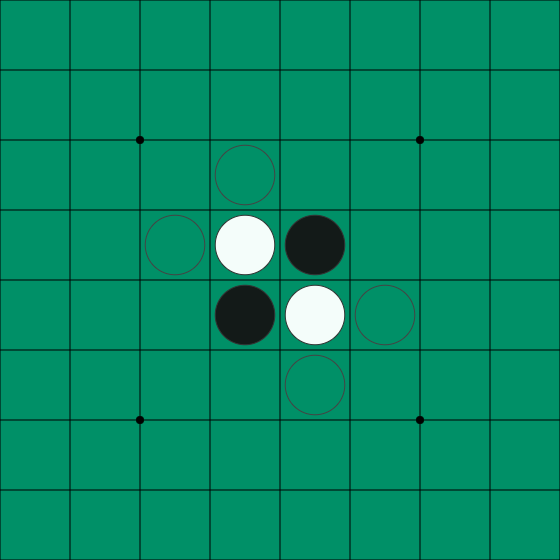
\includegraphics[width=0.7\textwidth]{ressources/plateau_init.png}
    \caption{Configuration initiale du plateau de jeu. Source : \href{https://www.eothello.com/}{eOthello}.}
    \label{fig:init_board}
\end{figure}

Elle s'encode comme suit. '0b', '0x' indiquent respectivement un nombre binaire et hexadécimal ; les underscores sont là pour faciliter la lecture :
\newline \newline
\noindent Le plateau noir : 
\begin{align*}
0b00000000\_00000000\_00000000\_00001000\_00010000\_00000000\_00000000\_00000000 \\
\end{align*}
Le plateau blanc :
\begin{align*}
0b00000000\_00000000\_00000000\_00010000\_00001000\_00000000\_00000000\_00000000 \\
\end{align*}
Ces deux entiers peuvent être réécris en hexadécimal pour une meilleure lisibilité :
\begin{align*}
    &0x00\_00\_00\_08\_10\_00\_00\_00 \quad (noir)\\
    &0x00\_00\_00\_10\_08\_00\_00\_00 \quad (blanc)\\
\end{align*}

Il est possible de récupérer la valeur d'une case $c_{i,j}$ d'un bitboard $b$ en utilisant la formule suivante : 
\begin{align*}
    (b\quad \gg\quad (8\times i+j))\quad \&\quad 1
\end{align*}
Avec $i$ la ligne, $j$ la colonne, $\gg$ l'opérateur de décalage à droite, et $\&$ l'opérateur logique 'et'.

Similairement, nous pouvons définir une case $c_{i,j}$ d'un bitboard $b$ en utilisant la formule suivante :
\begin{align*}
    b\quad |\quad (1\quad \ll\quad (8\times i+j))
\end{align*}
Avec $\ll$ l'opérateur de décalage à gauche, et $|$ l'opérateur logique 'ou'.

Nous obtenons toutes les pièces posées et toutes les cases vides avec les opérations logiques suivantes :
\begin{align*}
    &\text{pieces} = \text{noir} \quad | \quad \text{blanc} \\
    &\text{vides} = \sim \text{pieces}
\end{align*}
Avec $\sim$ l'opérateur logique 'non'.

De manière générale, n'importe quel pion ou coup peut être ajouté au plateau avec l'opérateur logique 'ou'.


\section{Algorithmes}
\label{sec:algo}

\subsubsection{Comment décaler un bitboard ?}
\label{subsec:shift}
Le calcul des coups valides est une étape cruciale pour le jeu, c'est par ailleurs l'étape la plus couteuse en temps de calcul. La représentation en bitboards nous permet de calculer les coups valides de manière très efficace, en vectorisant les opérations. Il est en effet possible de calculer simultanément les coups valides qui sont dans la même direction, en utilisant des masques prédéfinis. 

Pour cela, il va nous falloir être capable de décaler un plateau entier dans les 8 directions cardinales. Nous le faisons en utilisant des opérations logiques, comme le montre le pseudo-code ci-après.
\begin{algorithm}
    \caption{Opérations de décalage pour les coups valides.}
    \begin{algorithmic}[1]
    \Function{Nord}{$x$}
        \State \Return $x \gg 8$
    \EndFunction
    
    \Function{Sud}{$x$}
        \State \Return $(x \,\, \& \,\, 0x00ffffffffffffff) \ll 8$
    \EndFunction
    
    \Function{Est}{$x$}
        \State \Return $(x \,\, \& \,\, 0x7f7f7f7f7f7f7f7f) \ll 1$
    \EndFunction
    
    \Function{Ouest}{$x$}
        \State \Return $(x \,\, \& \,\, 0xfefefefefefefefe) \gg 1$
    \EndFunction
    \end{algorithmic}
    \label{alg:shift_ops}
\end{algorithm}

Les masques permettent d'éviter un débordement ou \textit{overflow}, une sortie de plateau, et de préserver les bords. Ils consistent à mettre à 0 les bits qui sont des positions sensibles dans la direction donnée. Nous obtenons ensuite $Nord-Est$, $Nord-Ouest$, $Sud-Est$, $Sud-Ouest$ en combinant les opérations précédentes. (Voir appendix \ref{app:logical_ops} pour plus de détails, ainsi que les codes python correspondant).

\subsection{Trouver les coups valides}
\label{subsec:valid_moves}

\subsection{Jouer un coup}
\label{subsec:play}

